\documentclass[main.tex]{subfiles}
\begin{document}

\section{Results and Performance Comparisson}\label{sec:results}
\subsection{Energy Deposition}

The analog and the digital setup were run with different amplitude thresholds, so in order to properly compare them the correct threshold need to be found. Since the two setups have different cable lengths to the detectors they are not attenuated to the same extent, so the digital setup will need a significantly higher threshold than the analog setup in order to accept the same events. Figure \ref{fig:qdc_comp} top panel shows the energy and time of flight spectra. It is clear from the energy spectrum that the digital setup has a lower threshold applied In addition to this the analog setup reaches the limit of the QDCs range slightly above \SI{6}{\MeV}$_\text{ee}$, whereas the digital spectrum continues. 

\begin{figure}[h]
    \centering
        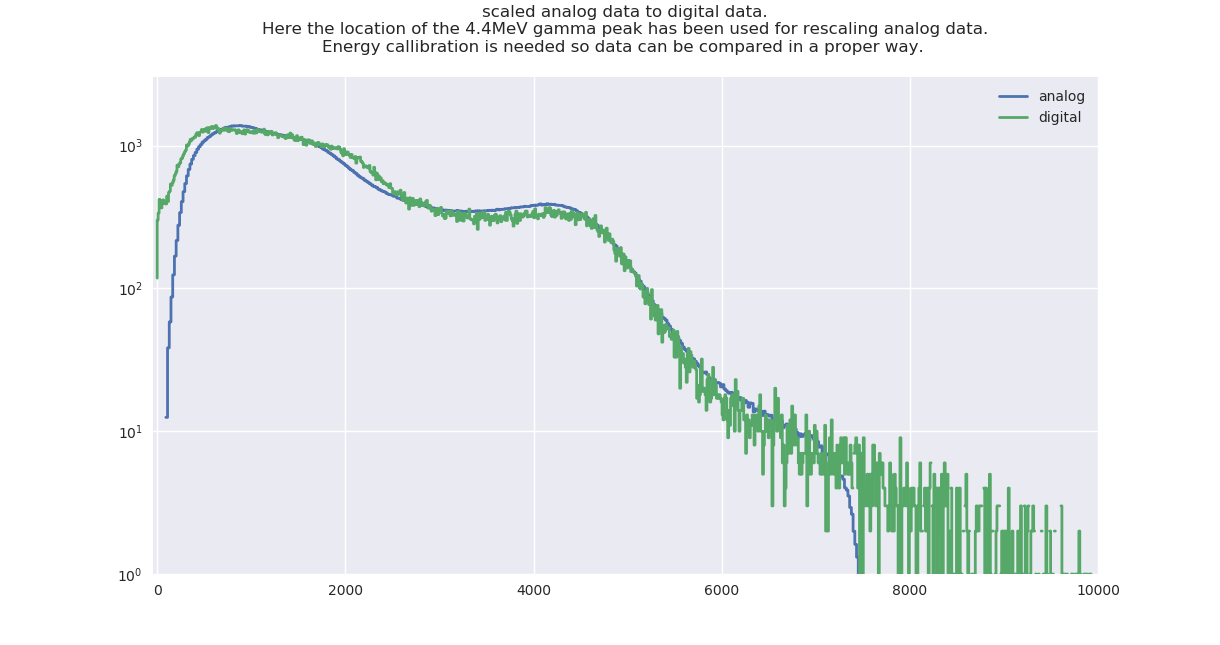
\includegraphics[width=0.8\textwidth]{CompareResults/qdc_comp.pdf}
        \caption{Comparison of analog and digital time of flight spectra. In the lower panel livetime has been taken into account and the digitized data has had a higher threshold enforced on the NE213 signals.}
    \label{fig:qdc_comp}
\end{figure}

In the bottom panel of the figure the threshold has been adjusted to match the analog setup and the counts of the analog setup have been rescaled to compensate for 56\% deadtime. The data acquisition software WaveDump does not offer a way to calculate deadtime\footnote{Although it is possible to make custom software that does this using CAENs libraries}, so instead the digitized data has been scaled to match the data from the analog daq. By carrying out these changes the two energy spectra look more alike, although the \SI{4.44}{\MeV}$_\text{ee}$ Compton edges look quite different. This may be because some of the high energy gamma rays were outside of the dynamic range of the digitizer.

Figure \ref{fig:qdc_ratio} shows the ratio between the digital and analog Energy spectra from after livetime adjustments and threshold alignment. Below \SI{0.8}{\MeV}$_\text{ee}$ the analog setup will pull the ration down due to the pedestal injection and above \SI{6}{\MeV}$_\text{ee}$ the ratio blows up because this is outside the range of the analog QDC modules. Ideally however everything inbetween 0.8 and \SI{6}{\MeV}$_\text{ee}$ should be very close to 1. Initially this seems to be the case, but near the \SI{4.44}{\MeV}$_\text{ee}$ compton edge there is a bump followed by a vally. This is likely because the highest amplitude digitized pulses were clipped, causing them to be pushed to lower values of deposited energy.
\begin{figure}[h]
    \centering
        \includegraphics[width=0.8\textwidth]{CompareResults/QDC_ratio.pdf}
        \caption{Ratio of the digital and analog QDC spectra.}
    \label{fig:qdc_ratio}
\end{figure}

\subsection{Time of Flight Spectra}
Like the energy spectrum the time of flight is heavily influenced by the choice of amplitude threshold. Figure \ref{fig:tof_comp} top panel shows the time of flight spectra for the two setups with the intial 49 mV NE213 threshold on the digital setup and 94.6 mV on the analog setup. Interestingly it seems that the analog setup is cutting away the slower neutrons (this does not mean that they are not \textit{fast} neutrons) by setting the amplitude threshold too high. By applying the new NE213 threshold of 151 mV to the digital setup and adjusting the livetime of both setups in the same manner as for the energy spectrum the time of flight spectrum shown in the bottom panel of figure \ref{fig:tof_comp} is obtained. A couple of things stand out here. First and foremost there are more counts in the digitized time of flight spectrum. This is because the YAP thresholds have not been aligned. Secondly the neutron peaks now have roughly the same shape, which means that the amplitude cut has removed the slower of the fast neutrons. Additionally, with a full width at half maximum of the gamma peak of \SI{7.67}{\ns} the analog setup seems to have a poorer time resolution than the digital setup which has a FWHM of 2.75 ns at the gamma peak.

\begin{figure}[h]
    \centering
        \includegraphics[width=0.8\textwidth]{CompareResults/tof_comp.pdf}
        \caption{Comparison of analog and digital time of flight spectra. In the lower panel livetime has been taken into account and the digitized data has had a higher threshold enforced on the NE213 signals.}
    \label{fig:tof_comp}
\end{figure}

\subsection{PSD Figure of Merit}
By fitting Gaussian functions to the neutron and gamma distribution shown in \ref{fig:fom_analog} and \ref{fig:fom_digital} one can express the quality of separation between the two distribution as a figure of merit, FoM, defined in terms of the centers, C, of the gaussians and their full width half maximum. This way of parametrizing the quality of a PSD method requires that the distributions are approximately Gaussian. This assumption appears to be valid for the neutron distribution, centered at 0.3, but both figure \ref{fig:fom_analog} and figure \ref{fig:fom_digital} shows a tail on the gamma distribution which is not matching with the fit. The assumption of Gaussian distributions is not valid for the distributions produced by the CNN method, so the FoM will only be used for comparing the charge comparison methods. 

In order to fit the Gaussians the raw PS histograms were first smoothened with a Gaussian kernel, which made it possible to locate extreme values. The Gaussians were then fitted. The two distributions are clearly better separated for the digital setup than for the analog setup. 

\begin{equation}
FoM = \frac{C_n - C_\gamma}{FWHM_n + FWHM_\gamma}
\end{equation}

\begin{figure}[ht]
	\begin{subfigure}[b]{\textwidth}
	    \centering
    	    \includegraphics[width=0.8\textwidth]{CompareResults/FOM_analog.pdf}
        	\caption{Analog setup}
	    \label{fig:fom_analog} 
	\end{subfigure}
	\begin{subfigure}[b]{\textwidth}
    	\centering
        	\includegraphics[width=0.8\textwidth]{CompareResults/FOM_digital.pdf}
        	\caption{Digital setup}
    	\label{fig:fom_digital} 
    \end{subfigure}
    \caption{The blue histograms shows the pulse shape parameter. The green curve is this same histogram after being smoothed by a Gaussian kernel, to allow for identification of extreme values. The red and green curves are fits to the gamma ray and neutron distributions respectively. The inserts show the pulse shape parameter as a function of energy, for full size version see fig \ref{fig:psd_a} and \ref{fig:psd_d}. }
\end{figure}

Looking at the inserts in both figures it can be seen that the FoM is highly energy dependent. This energy dependence is illustrated by figure \ref{fig:psd_fom_trend}. The digital setup performs better at all energy thresholds and only at \SI{3}{MeV} the analog reaches the FoM the digital setup had at \SI{0.4}{\MeV}. The ideal placement of the pulse shape discrimination cut also varies with energy, but as is shown in figure \ref{fig:psd_cut_trend} the linearizations of the pulse shape parameters have minimized these variations.
\begin{figure}[ht]
	\begin{subfigure}[b]{\textwidth}
	    \centering
    	\includegraphics[width=0.8\textwidth]{CompareResults/PSD_comp.pdf}
        \caption{}
	    \label{fig:psd_fom_trend} 
	\end{subfigure}
	\begin{subfigure}[b]{\textwidth}
    	\centering
        \includegraphics[width=0.8\textwidth]{CompareResults/PSD_cut.pdf}
        \caption{}
    	\label{fig:psd_cut_trend} 
    \end{subfigure}
    \caption{(a) Pulse shape discrimination figure of merit plotted as a function of minimum deposited energy. (b) Ideal pulse shape cut as a function of minimum deposited energy.}
\end{figure}


\subsection{Misclassification rate}
Another way to compare the performance of the PSD methods is by estimating the misclassification rate. This can be done by evaluating the time of flight spectrum in three different regions and comparing the relative number of neutron and gamma ray labeled events. Ideally the number of gamma rays identified per nanosecond channel in the background region should be the same as the number of gamma rays identified in the neighborhood of the neutron time of flight peak. Likewise the number of neutrons identified at the gamma peak should correspond to the neutron background.

This definition of misclassificaton rate is relying on the assumption that the background is approximately flat and that it has been determined fairly successfully.

Figure \ref{fig:tof_cc_cnn} shows the time of flight spectrum obtained with the analog setup filtered according to the charge comparison method, as well as the spectrum obtained from the digital setup, filtered by charge comparison and by the CNN. Gamma rays are colored blue, neutrons red and their intersection is purple. 

For the analog setup a high degree of contamination is evident. From \ref{fig:tof_ps_a} it was found that a number of the injected YAP start triggers remained even after cutting away events below \SI{0.8}{\MeV}, and that these landed at the gamma ToF but with very high PS values. These events will be part of the reason why there is nearly 12\% misclassification near the gamma peak.

The digital setup provides a lower misclassification rate with the charge comparison method, at \textgamma-n region: 10.96\% error and \textgamma-\textgamma\; region : 3.56\% error. The CNN approach reaches even better results with \textgamma-n region: 6.53\% error and \textgamma-\textgamma\; region : 2.63\% error.

The neutron background is found to be nearly the same by the analog and digital charge comparison methods, at 37.32\% and 38.38\% respectively. The CNN method finds a significantly higher background of neutron events at 44.05\%. 

The correct fraction of events due to neutrons interacting in the NE213 is not trivial to determine. Although the source is approximately isotropic radiation scattered by the aquarium and walls of the room complicates matters. So to get a better idea of what fraction of neutrons to expect simulations are needed. It is however clear that the CNN distribution is better at reproducing a flat background of neutrons at the gamma peak and vice versa, than the digital and analog charge comparison methods, so it seems likely that 44.05\% is a better estimate.

------------------------------------------------

NOTES: If a model is biased towards a certain particle species, then the background will also be incorrect. In this way one can minimize the classification error for one species by having a model biased in favor of this species. This will however cause the classification error for the other species to grow. perhaps it is better to use $\sqrt{error_\gamma^2+error_n^2}$.



\begin{figure}
    \centering
    \begin{subfigure}[bh]{\textwidth}
   	   	\centering
	    \includegraphics{AnalogResults/ToF_filt.pdf}
        \label{fig:ToF_filt_A}
    	\caption{Time of flight spectrum filtered by a linear cut at PS = 0.259.}
    	\label{fig:ToF_filt_A}
   	\end{subfigure}
    \begin{subfigure}[bh]{\textwidth}
   	    \centering
        \includegraphics{DigitalResults/ToF_filt.pdf}
        \caption{Time of flight spectrum filtered by a linear cut at PS=0.222.}
        \label{fig:ToF_filt_D}
    \end{subfigure}
	\begin{subfigure}[bh]{\textwidth}
	    \centering
        \includegraphics{DigitalResults/CNNToF_filt.pdf}
        \caption{Time of flight spectrum filtered by a linear cut at prediction = 0.5.}
        \label{fig:ToF_filt_D_CNN}
    \end{subfigure}
	
	\caption{}
    \label{fig:tof_cc_cnn}
\end{figure}






\end{document}